\chapter{Analyse}
\label{Analyse}
Im folgenden Kapitel wird die Analyse der Netzwerksicherheit in Industrie 4.0 Umgebungen durchgeführt. Zuerst wird eine Beschreibung und Einordnung der Bedrohungen von Industrie 4.0 Systemen anhand der in \autoref{Grundlagen:Grundprinzipien der sicheren Kommunikation} genannten Schutzziele und der aktuellen Industriestandards \autoref{Grundlagen:Normen und Standards} durchgeführt. Anschließend werden, aufgrund der bestehenden Infrastruktur und der Heterogenität der Netzwerklandschaft der Industrie, verschiedene Integrationsansätze für einen standardisierten Datenaustausch beschrieben. Die dabei etablierten Techniken und Protokolle des \ac{IoT} und \ac{IIoT} sowie neue \ac{M2M} Kommunikationswege der Industrie 4.0 werden dann nach den Schichten des \ac{TCP}/\ac{IP} Referenzmodells untersucht, um eine strukturierte Vorgehensweise zu ermöglichen und ein ganzheitliches Bild der Netzwerkkommunikation zu erhalten. Die Analyse wird mit Hilfe des Industrie 4.0 Testsystems (\cite{Weber2018}) durchgeführt. Dieses wird genutzt und erweitert, um unterschiedliche Szenarien darzustellen und die Sicherheit der Netzwerkkommunikation mit Hilfe verschiedener Softwaretools und Vorgehensweisen zu analysieren.

\section{Bedrohungen}
\label{Analyse:Bedrohungen}
Die vierte industrielle Revolution, das \ac{IIoT} und dessen Vielzahl an aktiven und passiven Elementen stellen in ihrer Komplexität eine große Herausforderung für die IT-Sicherheit dar. Einerseits muss die Sicherheit der laufenden Software, der Infrastruktur, Anwendungs- und Rechnersysteme gewährleistet werden, andererseits muss die Betriebssicherheit der Geräte und Anlagen, welche mit dem Internet verbunden sind sichergestellt werden. Das Management der IT-Sicherheit in Industrie 4.0 Netzen geht über Unternehmensgrenzen hinweg, da Netze und Systeme für Kunden, Lieferanden und Partner bereitgestellt werden (\cite{DTAG2016}). Somit hat sich auch die Bedrohungslage der Netze geändert. Das \ac{BSI} beschreibt die Top 10 Bedrohungen und deren Folgen für \ac{ICS} in \cite{ICSSec2016}.

\begin{enumerate}
    \item Social Engineering und Phishing
    \item Einschleusen von Schadsoftware über Wechseldatenträger und externe Hardware
    \item Infektion mit Schadsoftware über Internet und Intranet
    \item Einbruch über Fernwartungszugänge
    \item Menschliches Fehlverhalten und Sabotage
    \item Internet-verbundene Steuerungskomponenten
    \item Technisches Fehlverhalten und höhere Gewalt
    \item Kompromittierung von Extranet und Cloud Komponenten
    \item \ac{DoS} und \ac{DDoS}
    \item Kompromittierung von Smartphones im Produktionsumfeld
\end{enumerate}

TODO - Einordnung - Bezug auf Analyse

Um die in \autoref{Grundlagen:Grundprinzipien der sicheren Kommunikation} genannten Schutzziele umzusetzen, ist es notwendig einen größtmöglichen Schutz gegen diese Bedrohungen bereitzustellen. Die Sicherheit eines Gesamtsystems kann nicht nur an einer einzigen Stelle im Kommunikationsstack hergestellt und gewährleistet werden. Es müssen alle Stellen des Kommunikationsstacks gegen Bedrohungen abgesichert werden (\cite{sichKom2017}). Dafür müssen die Netzwerkinfrastruktur und die eigentliche Kommunikation im Netzwerk gesichert werden. Dies geschieht durch die Abschottung von Systemen, die Einschränkung von Zugangsberechtigungen, die Härtung der Sicherheit der genutzten Komponenten sowie den Einsatz von geeigneten Netzwerkprotokollen und Verschlüsselungsverfahren.

\section{Integrationsansätze}
Die Grundlage der Industrie 4.0 Kommunikation ist ein standardisierter Datenaustausch über alle Schichten der Automatisierungspyramide hinweg. Dabei stellt der \ac{IEC}-Standard \ac{OPC UA} einen vielversprechenden Ansatz für einen standardisierten Informationsaustausch über Unternehmensgrenzen hinweg dar. Jedoch müssen auch bestehende Systeme in die Industrie 4.0 Kommunikation integriert werden. Dies führt häufig zu Problemen, da diese Systeme proprietäre Protokolle nutzen, besondere Anforderungen wie Echtzeitkommunikation besitzen oder gar keine Schnittstelle bereitstellen. Es bestehen grundsätzlich zwei Ansätze zur Integration dieser Anlagen. TODO - ref.

\subsection{Konsolidierung der Netzwerkkommunikation}
TODO - Eine Möglichkeit der Entwicklung zu einer Smart Factory ist die Konsolidierung die Netzwerkkommunikation. Fokus auf OPC UA, da standardisiert.
TODO - neue Netze/Factories können so geplant werden, dass die Maschinen die benötigten Schnittstellen bereitstellen.
Ansatz: teuer, aufwendig bzw. nicht möglich, da embedded System bzw. keine Ressourcen oder keine Schnittstellen

\subsection{Gatewaykommunikation}
Eine Alternative zur Umstellung der bestehenden Systeme stellt die Kommunikation über Gateways dar. Hierbei gibt es mehrere Softwarelösungen, welche unterschiedliche Ziele verfolgen. Es werden Systeme zur Anlagenoptimierung (TODO - ref. SePiA.Pro), der Bereitstellung einer offenen, branchenübergreifenden Plattform mit diversen Smart Services wie Datenanalyse und Flottenmanagement (TODO - ref. Siemens Mindsphere, DeviceInsight) und dem herstellerübergreifenden Gerätemanagement (AXOOM) entwickelt \cite{acatec2016}. Die Systeme sammeln und verwalten die Daten der Anlagen an zentraler Stelle und stellen sie im Netzwerk zur Verfügung. Der Einsatzmöglichkeiten dieser Softwarelösungen sind von den vorhandenen Schnittstellen der Anlagen abhängig und benötigen eine individuelle Konfiguration um den unterschiedlichen Anforderungen der Industrielandschaft gerecht zu werden.

TODO - Im folgenden Abschnitt wird die Umsetzung der Kommunikation über eine digitale Serviceplattform am Beispiel von AXOOM dargestellt. eher nicht!

\subsubsection{AXOOM}
TODO - 2016 Innovationspreis deutsche Indsutrie
TODO - unterstützt Optimierung der Wertschöpfungskette -> ERP-, MES Kommunikation über "bekannte", offene Schnittstellen (REST usw.) 
TODO - unterstützt Anbindung von \ac{IoT}. Analyse und Visualisierung von Daten -> Kommunikation über spezielle Schnittstellen
TODO - sichere Kommunikation durch AXOOM Gate - wie? Quellen? -> "Dieses basiert teilweise auf Technologien unseres Partners C-Labs und schafft eine direkte Verbindung zwischen dem Kundennetzwerk und der Cloud. Das AXOOM Gate ist in der Lage, Daten herstellerunabhängig von allen angebundenen Geräten zu sammeln, so dass diese verschlüsselt an die AXOOM Plattform gesendet und dort visualisiert und ausgewertet werden können. Besonderen Schutz bei der Datenübertragung bietet ein mehrstufiges Sicherheits- und Verschlüsselungskonzept auf Komponenten-, Transport-, Applikations- und Anwenderebene. So wird eine genaue Zugriffskontrolle innerhalb der Fabrik sowie auf die Fabrik sichergestellt, unsichere Verbindungen von und nach Außen sind ausgeschlossen."
TODO - offene Schnittstellen für Low Level
TODO - REST usw. für High Level Applications
TODO - Softwareschwachstellen, Softwarefehler 
TODO - Herstellerabhängigkeit
TODO - Kosten der Interfaceentwicklung, usw.
TODO - AXOOM Absatz unnötig

\section{Netzzugangsschicht}
Die Netzzugangsschicht stellt die erste Instanz der Kommunikation in einem Netzwerk dar. Sie beinhaltet das Übertragungsmedium sowie die Topologie, in welcher die Kommunikation stattfindet. Das Übertragungsmedium bestimmt die Form der Signalübertragung. In Industrie 4.0 Netzen können neben der klassischen Kabelverbindung auch andere (instabile) Kanäle wie Mobilfunk oder Satelliten in Frage kommen. Um die Kommunikation über alle Medien sicher und zuverlässig zu gestalten, müssen auf technischer Ebene Protokolle genutzt werden, welche es ermöglichen die gegebenen Schutzziele zu realisieren und die Integrität der Daten bei der Übertragung über große Entfernungen zu gewährleisten. Dominante Technologien dieser Schicht sind \ac{IEEE} 802.3 (Ethernet)\footnote{Link zu IEEE 802.3}, \ac{IEEE} 802.11 (Wireless LAN)\footnote{Link zu IEEE 802.11} und \ac{IEEE} 802.15.4\footnote{Link zu IEEE 802.15.4} (\cite{sichKom2017}).

Aus zeitlichen Gründen wird keine weitere Analyse der verschiedenen Übertragungsmedien und deren Protokolle durchgeführt und sich im Rahmen dieser Thesis auf die Analyse von kabelgebundenen Ethernet-basierten Netzen, deren Topologie und Kommunikation beschränkt.

\subsection{physikalischer Zugang}
Die Netzzugangsschicht beinhaltet als einzige Schicht des \ac{TCP}/\ac{IP} Referenzmodells nicht nur die verwendeten Protokolle zur Signalübertragung, sondern auch die physikalischen Gegebenheiten des Übertragungsmediums. Die Sicherheit dieser Netzwerkschicht beinhaltet somit nicht nur die verwendeten Techniken, sondern auch die physische Sicherheit der Systeme. Sie wird durch den Zugang zur Hardware dargestellt und besitzt eine große Bedeutung, um unbefugte Eingriffe in das Netzwerk zu verhindern. Die Sicherheit dieser Systeme wird durch die physikalische Abschottung mit Hilfe von abschließbaren Serverschränken, genereller Zugangskontrolle sowie der Abschaltung von Ports an Netzwerkkomponenten oder Endsystemen gewährleistet. (\cite{sichKom2017})

\subsection{Topologie}
Die Topologie eines Netzwerks bestimmt den physikalischen Weg der Netzwerkpakete über die Leitungen. In der Industrie werden je nach Anwendungsfall verschiedene Topologien, wie Punkt-zu-Punkt-, Bus-, Stern- oder auch Hybride-, zur Kommunikation im Netzwerk genutzt. Jede dieser Netzstrukturen bietet Vor- und Nachteile bzgl. Durchsatz, Administrationsaufwand und Skalierbarkeit (\cite{burke2013}). Um die Grundidee der Industrie 4.0, die unternehmensübergreifende, intelligente Vernetzung von Produktionsressourcen umzusetzen, ist eine einheitliche Kommunikation notwendig. Industrie 4.0 Netze kommunizieren über \ac{TCP}/\ac{IP} Verbindungen und basieren auf dem \textit{Ethernet}\footnote{Link zu IEEE Ethernet} Protokoll. Sie werden in über Gateways miteinander verbundenen Sterntopologien realisiert. Die Topologie eines Netzwerks bietet Schnittstellen, um Einfluss auf das Netzwerk zu nehmen. Selbst unbefugter Zugriff auf der untersten Schicht des \ac{TCP}/\ac{IP} Referenzmodells kann die Sicherheit der Datenübertragung oder die Funktionsweise des Netzwerks beeinträchtigen.

TODO - Beschreibung von Angriffen durch Eingriff auf Hardware; Verweis auf Anwendungsszenario in Internetschicht.
TODO - Ansatz: Berechnung von Latenzzeiten, RTT, Auswirkungen aufzeigen, Congestion Window, Sliding Window

\subsection{\ac{VLAN}}
\label{Analyse:VLAN}
TODO - Taggen von Frames, da keine Kommunikation im Schichtenmodell zwischen den Schichten stattfindet. Somit QoS schwierig, da es von allen Hardwarekomponenten unterstützt werden muss und nicht nur auf Anwendungsebene funktionieren kann.

\subsection{\ac{ARP}}
\label{Analyse:ARP}
TODO - praktisch nur wenn Tool vorhanden ist.

\subsection{vertikale Integration bestehender Komponenten}
TODO - Feldbus, SPS, Anlagensteuerung (SCADA) -> Bindeglied zu IP-Netzen
TODO - Ansatz: OPC UA Clients sind Gateways in Testumgebung -> Verweis auf Analyse in höheren Schichten
TODO - Vieles in Praxis nicht umsetzbar darum größtmöglicher Schutz durch Abschottung.

\section{Internetschicht}
Auf der Internetschicht findet die Vermittlung der Datenpakete zwischen den Teilnehmern im Netzwerk statt. Auf dieser Schicht hat sich, mit dem Siegeszug des Internets, \ac{IP} zum Standard für Netzwerkübergreifende Rechnerkommunikation durchgesetzt (\cite{meinel2011}). Dies gilt auch für die immer komplexer werdenden Industrienetzwerke und die Industrie 4.0.

Zu den Aufgaben der Internetschicht gehört das Bereitstellen von Adressen, das Routing, die Fragmentierung von Datenpaketen zur Übertragung im Netzwerk sowie die Sicherstellung der Dienstgüte. Um Routing und Adressvergabe in \ac{IP}-Netzen zu realisieren, werden die Dienste \ac{DNS} (\autoref{Analyse:DNS}) und \ac{DHCP} (\autoref{Analyse:DHCP}) genutzt. Das \ac{IPAM} und die Zuordnung der physikalischen Hardware zur logischen \ac{IP}-Adresse erfolgt mit Hilfe des \ac{ARP}. Da die Kommunikation in einem \ac{IP}-Netz ohne diese Dienste und Protokolle nicht möglich ist, stellen sie einen wichtigen Bestandteil im Netzwerk dar und müssen vor Sabotage geschützt werden. 

\subsection{\ac{QoS}}
Eine Industrie 4.0 Netzwerkinfrastruktur kann aufgrund der unterschiedlichen Anforderungen an die Systeme auf verschiedenste Weisen ausgeprägt sein. Die Heterogenität der Komponenten im Netzwerk und deren Anforderungen an die Kommunikation auf der vertikalen Ebene der Automatisierungspyramide \autoref{Grundlagen:Automatisierungspyramide} stellen eine Herausforderung für die Sicherheit der Datenübertragung dar und können die Umsetzung eines Netzwerks beeinflussen. Des Weiteren erstrecken sich Industrie 4.0 Umgebungen über weite Distanzen (\ac{MAN}, \ac{WAN}, \ac{GAN}) und sind somit auch von physikalischen Gegebenheiten wie Latenz und Jitter betroffen. Diese Erscheinungen müssen berücksichtigt werden, um eine fehler- und verlustfreie, sichere Kommunikation zu gewährleisten \cite{torscht2014}.

Für die Beurteilung und Bereitstellung der Dienstgüte in \ac{IP}-Netzen müssen die Übertragungsgüte der Netzzugangsschicht sowie die übertragungstechnischen Parameter der Internetschicht (\ac{IP}-Ebene) betrachtet werden. In IP-Netzen wird der Einfluss auf die \ac{QoS} in den folgenden Parametern beschrieben:
\begin{itemize}
    \item Latenzzeit: Dauer der Paketübertragung
    \item Jitter: Abweichung der Latenzzeit von ihrem Mittelwert
    \item Paketverlustrate: Wahrscheinlichkeit des Verlusts von IP-Paketen während der Übertragung
    \item Durchsatz: gemittelte Datenmenge pro Zeiteinheit
\end{itemize}
All diese Faktoren haben in einem paketorientierten Netzwerk, in welchem die Datenpakete nach dem \textit{Best-Effort-Prinzip} versendet werden, auf die fehlerfreie Kommunikation aufgrund der durch \textit{Ethernet} und \ac{IP} bereitgestellten Fehler- und Flusskontrolle wenig Einfluss. Sie spielen jedoch bei zeitkritischen Anwendungen der Industrie 4.0 eine wichtige Rolle. Auf den niedrigeren Schichten des \ac{TCP}/\ac{IP} Referenzmodells ist es nicht möglich zwischen verschiedenen Datenpaketen der höheren Schichten zu unterscheiden. Um dieses Problem zu lösen werden auf Dienste mit besonderer Güte in \ac{VLAN}s aufgenommen und somit deren Pakete bereits auf der Netzzugangsschicht kenntlich gemacht (\autoref{Analyse:VLAN}), um die Dienstqualität sicherzustellen. Des Weiteren müssen, um \ac{QoS} in einem Netzwerk anzuwenden, diese Mechanismen auf der gesamten Übertragungsstrecke implementiert werden. Der Transport von Daten unterschiedlicher Priorität in Netzwerken wird in \ac{IEEE} 802.1p und \ac{IEEE} 802.1Q\footnote{IEEE Std 802.1Q - IEEE Standard for Local and metropolitan area networks--Bridges and Bridged Networks} beschrieben.

\subsection{IPsec}
TODO - Die Internetschicht bietet mit IPsec eine Möglichkeit den Datenfluss, im Vergleich zu anderen Verschlüsselungsverfahren, bereits auf der Internetschicht des \ac{TCP}/\ac{IP} Referenzmodells zu sichern.

\section{Transportschicht}
\label{Analyse:Transportschicht}
Während auf der Netzwerkschicht allein das Protokoll \ac{IP} die Basis für die Vernetzung und Adressierung von Industrie 4.0 Systemen darstellt, wird das Protokoll der Transportschicht durch die Anforderungen an das Netzwerk bestimmt. Der wesentliche Teil der Kommunikation in der Industrie 4.0 erfolgt über ein \ac{IP} Netzwerk, welches zum Datentransport das Protokoll \ac{TCP} für \textit{End2End} (\autoref{Grundlagen:End2End}) Kommunikation nutzt (\cite{sichKom2017}). Wie in \autoref{Grundlagen:Kommunikationsstrukturen} beschrieben, bieten sich in der Praxis bei besonderen Anforderungen wie der Verteilung von Informationen im Netzwerk oder zeitkritischen Automatisierungsanwendungen jedoch auch andere Strukturen für die Kommunikation wie \textit{Publish-Subscribe} (\autoref{Grundlagen:Publish-Subscribe}) in Verbindung mit dem Datagramm \ac{UDP} an. 

Das Protokoll \ac{TCP} sowie das Datagramm \ac{UDP} sind für die Übertragung der Segmente im Netzwerk sowie das Multi-/Demultiplexing verantwortlich. Dabei spielt der Inhalt der zu übertragenden \textit{payload} keine Rolle. Die Analyse der Sicherheit im Netzwerk auf dieser Schicht des \ac{TCP}/\ac{IP} Referenzmodells beschränkt sich somit ausschließlich auf die Form der Datenübertragung sowie der dafür genutzten Netzlast.

\subsection{\ac{TCP}}
\label{Analyse:TCP}
Das Protokoll \ac{TCP}\footnote{\cite{TCP}} verfolgt das Prinzip eines \textit{guaranteed delivery} und stellt eine zuverlässige Datenübertragung zwischen zwei \textit{Hosts} (Unicast) bereit. Hierzu werden verschiedene Mechanismen zur Segmentierung der Daten, dem Verbindungsmanagement sowie der Fehler- und Flusskontrolle bereitgestellt. Diese Mechanismen, welche durch den Aufbau des des \ac{TCP} Headers und die Nutzung von Timeouts und Algorithmen realisiert werden, sind für den Erfolg des Protokolls für zuverlässige, paketorientierte \textit{End2End} Kommunikation verantwortlich.

Ein wichtiger Bestandteil des \ac{TCP} Verbindungsmanagements und der Fehlerkontrolle stellt der 3-Wege-Handshake beim Verbindungsaufbau sowie -abbau dar. Er wird mittels der \textit{Sequence-} und \textit{Acknowledgementnumber} sowie den zugehörigen \textit{Flags} des \ac{TCP} Headers (\ac{SYN}, \ac{SYN-ACK}, \ac{ACK}, \ac{FIN}) realisiert. Während des Verbindungsaufbaus werden die Adresse des Clients sowie der Status der Verbindung im Speicher gehalten. Die folgende Abbildung zeigt schematisch den Ablauf eines \ac{TCP} Verbindungsaufbaus zwischen Client und Server. Der Client sendet zuerst eine Paket mit SYN-Flag zum Server. Dieser bestätigt das eingetroffene Paket des Clients mit dem SYN-ACK Flag, inkrementiert die Sequenznummer x in seinem \textit{acknowledgment number} Segment\footnote{text} und erzeugt eine neue Sequenznummer für das Antwortpaket. Der Verbindungsaufbau wird durch die Bestätigung des SYN-ACK Pakets durch den Client und den Empfang des ACK Pakets vom Server abgeschlossen. Die initiale Sequenznummer x des SYN Pakets sowie die initiale Sequenznummer y des SYN-ACK Pakets können von den Beteiligten frei bestimmt werden.

\begin{figure}[h]
    \centering
    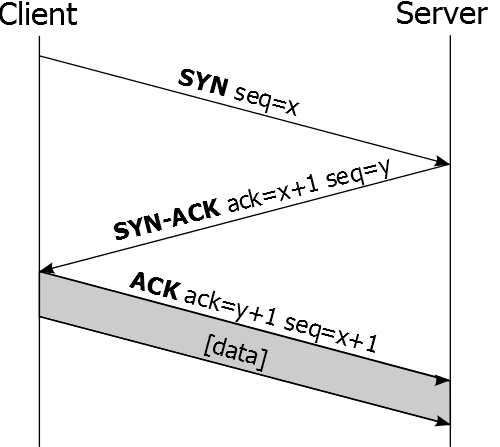
\includegraphics[width=10cm]{tcp-verbindungsaufbau}
    \caption{TCP Verbindungsaufbau}
    \label{Analyse:TCP Verbindungsaufbau}
  \end{figure}
  
\clearpage

\subsubsection{SYN-Flood}
Der Mechanismus des 3-Wege-Handshakes kann durch einen SYN-Flood Angriff ausgenutzt werden und somit die Netz- und Systemlast manipuliert werden. Der SYN-Flood stellt eine Form des \ac{DoS} bzw. \ac{DDoS} Angriffs dar. Dabei werden zu einem gezielten \ac{TCP} Dienst viele Pakete mit gesetztem SYN \textit{Flag} gesendet, um einen Verbindungsaufbau zum Server vorzutäuschen. Nach Erhalt des Pakets sendet der Server dem Client ein SYN-ACK Paket um den Verbindungsaufbau zu initiieren und wartet auf Bestätigung. Diese Bestätigung wird vom Angreifer unterschlagen. Somit bleiben auf dem angegriffenen System Ressourcen dieser halb offenen Verbindung bis zum erreichen eines Timouts belegt. Ein verteilter Angriff auf ein System kann dessen Ressourcen schnell komplett beanspruchen und somit zur Ablehnung jeglicher weiterer Verbindungen führen.

Die Kritikalität dieses Angriffs liegt in der Unausgewogenheit der benötigten Ressourcen zwischen Angreifer und Opfer. Es benötigt nur wenig Rechenaufwand und Bandbreite um ein 20 Byte großen \ac{TCP}-SYN Header mit entsprechender \textit{payload} zu erzeugen und zu versenden, jedoch viele Ressourcen um sich durch eine Echtzeitanalyse der Pakete durch eine Firewall oder SYN-Cookies vor diesen Angriffen zu schützen. Diese werden aufgrund ihrer Ressourcenbelastung aus wirtschaftlichen Gründen meist nur minimal oder gar nicht umgesetzt.

Der Mechanismus der SYN-Cookies wird auf dem Server implementiert. Hierbei werden in die initiale Sequenznummer des vom Server gesendeten SYN-ACK Pakets die Informationen Zeitstempel, \ac{IP} Adresse und Port von Client und Server kodiert, welche normalerweise in einer Tabelle im Speicher gehalten werden müssten. Somit ist ein überlaufen der Tabelle unmöglich, da sie nicht vorhanden ist. Jedoch benötigt jede Kodierung und Dekodierung Systemressourcen. Ein ausreichend großer Angriff auf das System kann somit trotzdem die gesamten Systemressourcen beanspruchen und somit das Ziel eines \ac{DDoS} Angriffs, die Negierung eines Dienstes, erfüllen.

Dedizierte Firewalls können mit Hilfe von \ac{IDS} die Pakete beim Eintreffen im Netzwerk analysieren, Angriffe erkennen und Verbindungen dieser Quelladressen blockieren.

\subsubsection{Sockstress}
Die Angriffsform Sockstress wurde im Jahr 2008 von den Sicherheitsforschern Jack C. Louis und Robert E. Lee von Outpost24\footnote{http://www.outpost24.com} entdeckt. Sie beinhaltet eine einfache Form eines \ac{DoS} Angriffs, welche den 3-Wege-Handshake des \ac{TCP} für unterschiedliche Angriffsszenarien manipuliert. Das Ziel dieses Angriffs ist, ähnlich wie beim SYN-Flood, eine Negierung eines Dienstes oder des gesamten Systems mit Hilfe asymmetrischer Ressourcenauslastung bei Angreifer und Opfer.

Im Gegensatz zu SYN-Flood stellt Sockstress eine Verbindung zum Server über den 3-Wege-Handshake her. In der einfachsten Form des Angriffs wird beim letzten \ac{TCP} Segment, welches vom Client zum Server während des 3-Wege-Handshakes übertragen wird, das \textit{Receive Window} Flag des Headers auf 0 gesetzt. Dies bedeutet, dass der Client dem Server mitteilt, dass er im Moment keine weiteren Daten empfangen kann. Der Server wird, durch den abgeschlossen Verbindungsaufbau, gezwungen die Verbindung im Speicher zu halten, offen zu lassen und den Client periodisch zu prüfen, ob dieser wieder Daten empfangen kann. Dies belegt Systemressourcen und kann genutzt werden, um einen Dienst oder ein System zum Ablehnen aller Verbindungen oder zum Absturz zu bewegen.

Da die Verbindungen zum Client zum Server vollständig aufgebaut werden, hat die Nutzung von SYN Cookies keine Auswirkungen auf den Erfolg dieses Angriffs. Industrieanlagen müssen mit Hilfe externer \ac{DDoS} Serviceanbieter wie Akamai\footnote{https://www.akamai.com} oder Cloudflare\footnote{https://www.cloudflare.com}, Firewalls und \ac{IDS} Systeme oder spezieller Appliances, welche den Netzwerkverkehr Netzwerk-, Transport- und Anwendungsschicht überwachen, geschützt werden.

Diese Form des \ac{DoS} Angriffs wurde am vorhandenen Industrie 4.0 Testsystem (\cite{Weber2018}) durchgeführt, um den Angriffsaufwand sowie die Auswirkungen auf die Systeme und Netzwerkkommunikation in Industrieumgebungen an einem Beispiel darzustellen (siehe \autoref{Impl:Sockstress}). 

TODO - In Abbildung XY ist zu erkennen - asymmetrischer Angriff - Monitoring Ressourcenauslastung - RAM bleibt nach dem Angriff weiterhin belegt -> nur Systemneustart gibt Speicher wieder frei 
TODO - Diagramm als Zusammenfassung der Implementierung
TODO - Ergebnisse beschreiben

\subsection{\ac{UDP}}
\ac{UDP}\footnote{Link - https://tools.ietf.org/html/rfc768} ist ein verbindungsloses\footnote{verbindungslos - TODO}, nicht-zuverlässiges\footnote{nicht zuverlässig - TODO} Übertragungsprotokoll. Der \ac{UDP} Header ist im Gegensatz zum \ac{TCP} Header (20 Bytes) nur 8 Byte lang und bietet somit einen sehr geringen \textit{Overhead}\footnote{Overhead - TODO} beim Versenden von \ac{IP} Paketen. \ac{UDP} wurde als Alternative zu \ac{TCP} entwickelt, um die Kommunikation mit niedrigeren Latenzen für Dienste wie \ac{SNMP} oder \ac{DNS}oder \ac{VoIP} zu ermöglichen (\cite{UDP2003}). Es wird auf den für die Latenz kritischen 3-Wege-Handshake verzichtet und das \textit{Fire-and-Forget}\footnote{Fire-and-Forget - TODO} Prinzip angewandt, wobei keine Verbindung zwischen zwei Kommunikationspartnern hergestellt wird, sondern die Pakete ohne Flusskontrolle vom Sender zum Empfänger gesendet werden.

\ac{UDP} findet in vielen Industrienetzen Einsatz als Transportprotokoll. Es bietet sich, vor allem durch seine Simplizität und den geringen Overhead im Netzwerk für die Informationsverteilung mit niedrigen Latenzzeiten an. Durch die Broad- und Multicast Funktionalitäten des \ac{UDP} ist es möglich über das Publish-Subscribe Pattern zu kommunizieren und somit die Netzlast bei eine großen Anzahl von Empfängern gering zu halten. Diese Form der Informationsverteilung über \ac{UDP} wird in \autoref{Analyse:OPCUA} mit Bezug auf das Protokoll \ac{OPC UA} analysiert.

\ac{UDP} führt keine Validierung der Absenderadresse im Paketheader durch (\cite{UDP2003}). Dies ermöglicht die Anwendung von \ac{IP} Spoofing. \ac{IP} Spoofing kann genutzt werden, um \ac{DoS} bzw. \ac{DDoS} Angriffe auf ein System durchzuführen. Eine Analyse des Netzwerkdienstes \ac{DNS}, welcher auf der Nutzung des Transportprotokolls \ac{UDP} basiert, wird in Kapitel \autoref{Analyse:DNS} beschrieben und durchgeführt.

\section{Anwendungsschicht}
\label{Analyse:Anwendungsschicht}
Die Netzwerkkommunikation der Anwendungsschicht in Industrie 4.0 Umgebungen basiert auf dem \ac{IP} der Internetschicht. Um die Integration und Verwaltung der Netzwerkteilnehmer zu erleichtern, werden \ac{IP} basierende Dienste wie \ac{DNS} für die Namensauflösung sowie \ac{DHCP} für die Adressvergabe und das Routing genutzt. Des Weiteren wird sie in Industrieumgebungen durch eine Vielzahl von Protokollen beschrieben. Bestehende Lösungen des \ac{IoT} nutzen Protokolle wie \ac{HTTP}, \ac{XMPP} oder \ac{SMTP} zur Kommunikation über das Netzwerk. In der \ac{M2M} Kommunikation des \ac{IIoT} haben sich die Protokolle und Standards \ac{OPC UA}, \ac{DDS}, \ac{MQTT} und \ac{CoAP} für unterschiedliche Anforderungen an die Netze und deren Teilnehmer hervorgetan. 

\subsection{\ac{DNS}}
\label{Analyse:DNS}
\ac{DNS} wird von der \ac{IETF} in den \ac{RFC} 1034\footnote{Domain Names – Concepts and Facilities}, 1035\footnote{Domain Names – Implementation and Specification}, 2181\footnote{Clarifications to the DNS Specification} und 2782\footnote{A DNS RR for specifying the location of services (DNS SRV)} beschrieben und verwaltet. Es stellt einen hierarchischen Verzeichnisdienst für \ac{IP}-Netze zur Verfügung. 

Eine der Hauptaufgaben des \ac{DNS} ist der \textit{forward lookup}. Hierbei werden Domain- bzw. Hostnamen in \ac{IP}-Adressen übersetzt. Das Zusammenspiel eines hierarchischen Verzeichnisdienstes und der Namensauflösung bietet Angriffsfläche zum Eingriff auf die Kommunikation im Netzwerk. Im folgenden werden bekannte Angriffsformen auf den \ac{DNS} Dienst und deren Auswirkungen auf das Netzwerk beschrieben.

\subsubsection{\ac{DNS} Spoofing}
Die Angriffsmethode des \ac{DNS} Spoofing verfolgt, wie \textit{Cache Poisoning}\footnote{Cache Poisoning - iwas}, das Ziel gefälschte \ac{RR} in den \ac{DNS} Cache des Opfers einzuschleusen. Während das \textit{Cache Poisoning} aus einer Softwareschwachstelle hervorging, bei der zusätzliche, gefälschte \ac{DNS} Einträge zu korrekten \ac{DNS} Antworten hinzugefügt wurden und somit der Cache eines Nameservers kompromittiert wird, befindet sich der Angriffsvektor beim \ac{DNS} Spoofing in der Fälschung von \ac{DNS} Antworten. Der Header der Netzwerkpakete werden mit Hilfe von \textit{IP Spoofing}\footnote{IP Spoofing bezeichnet das Versenden von IP Paketen mit gefälschter Absender-IP} so manipuliert, dass sie vorgeblich vom \textit{authorativen} Nameserver stammen. 

Um \ac{DNS} Spoofing erfolgreich durchzuführen muss die gefälschte \ac{DNS} Response des Angreifers vor der Antwort des zuständigen Nameservers beim angegriffenen \ac{DNS} Resolver eintreffen. Sobald der physikalische Zugang zum Netzwerk gewährleistet ist, können die Latenzzeiten der gefälschten Pakete im Netzwerk sehr gering gehalten werden. Ist dies nicht möglich, kann mit Hilfe eines \ac{DoS} bzw. \ac{DDoS} Angriffs auf den zuständigen Nameserver, dessen Antwortzeit beeinflusst werden. Des weiteren muss die ID im \ac{DNS} Header mit der des Request übereinstimmen. Dies kann am Testsystem am Beispiel der Namensauflösung des \ac{OPC UA} Discovery Servers mit Hilfe des Netzwerkanalysetools Wireshark\footnote{Link zu Wireshark} nachgewiesen werden.

\begin{figure}[h]
    \centering
    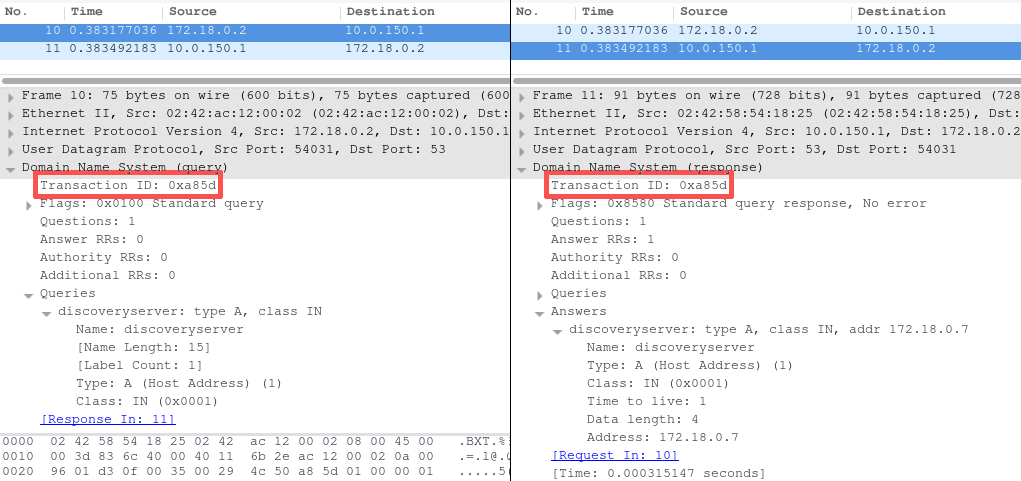
\includegraphics[width=15cm]{dns-response-request}
    \caption{Wireshark - ID im DNS Header}
    \label{Analyse:DNS Request Response}
  \end{figure}
  
\clearpage

In der Darstellung ist auf der linken Seite ein DNS Request des \ac{OPC UA} Discovery Servers und dessen DNS Header mit ID zu erkennen. Auf der rechten Seite ist die Antwort des im Netzwerk vorhandenen \ac{DNS} Nameservers zu sehen.

\subsubsection{\ac{DNS} Amplification}
Eine Form eines \ac{DDoS} Angriffs (\autoref{Analyse:DoS/DDos}) ist über \ac{DNS} möglich und wird \ac{DNS} Amplification genannt. Bei der \ac{DNS} Amplification werden \ac{DNS} Anfragen an offene Nameserver gesendet und mit Hilfe von \ac{IP} Spoofing als Quell-\ac{IP} die Adresse des Angreifers genutzt. Somit treffen die \ac{DNS} Antworten beim anzugreifenden System ein und belasten dieses durch erhöhten Rechenaufwand sowie dessen Netzwerk durch Traffic. Ein weiterer Seiteneffekt dieses Angriffs ist eine hohe Last der Nameserver, welches durch das rekursive Verhalten der \ac{DNS} Namensauflösung hervorgerufen wird. \ac{DNS} Amplification bezeichnet eine Form des \ac{DRDoS}.

Mit der Erweiterung des \ac{DNS} in der \ac{IETF} \ac{RFC} 2617\footnote{Link - https://www.ietf.org/rfc/rfc2671.txt} wurde es notwendig, die Größe der \ac{DNS} Antworten von 512 Byte auf einen dynamischen Puffer bis über 4000 Bytes zu erhöhen, um zusätzliche Informationen und Flags wie \autoref{Analyse:DNSSEC} über das \ac{DNS} übertragen zu können. Dies wird sich vom Angreifer zunutze gemacht, da an den Nameserver Requests mit einer Paketgröße von 60 Bytes gesendet werden können, welche eine Antwort mit 4000 Bytes und mehr provozieren und somit einen \ac{BAF} von ca. 66 im Netz haben. \cite{Ledermueller2009}. Der \ac{BAF} beschreibt das Verhältnis von Eingang- zum Ausgangssignal. Dies wird bei \ac{DNS} Amplifikation durch die Paketgröße der Anfrage sowie der Antwort dargestellt.

Die folgende Abbildung stellt einen \ac{DDoS} Angriff durchgeführt durch \ac{DNS} Amplification schematisch dar. Der Angreifer (links) sendet zu zwei offenen Nameservern gefälschte \ac{DNS} Anfragen mit Quelladresse des Opfers (rechts). Die offenen Nameserver erfragen beim authorativen Nameserver die Zone, dieser stellt die erfragten \ac{RR} bereit und die offenen Nameserver senden dem Opfer Antworten zu.

\begin{figure}[h]
    \centering
    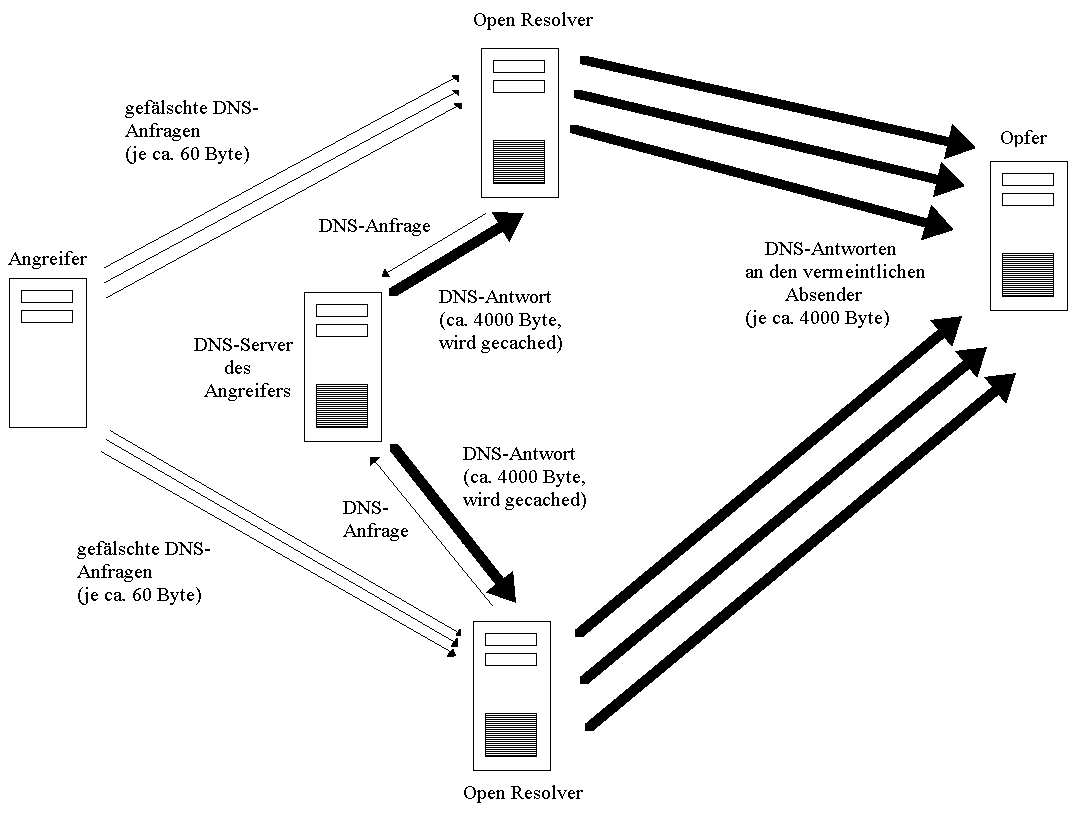
\includegraphics[width=15cm]{dns-amplification}
    \caption{Schematisches Beispiel: DNS Amplification}
    \label{Analyse:DNS Amplification}
  \end{figure}
  
\clearpage

Diese Form des Angriffs kann aus dem internen Netz sowie von extern auf öffentlich zugängliche Systeme durchgeführt werden. \ac{DoS} Attacken stellen besonders für Industrie 4.0 Netzwerke, deren komplexe Kommunikation und Anforderungen eine hohe Bedrohung dar. Durch den erheblichen \ac{BAF} können diese Angriffe mit wenig Bandbreite beim Angreifer durchgeführt werden und gleichzeitig das Netzwerk des Opfers voll auslasten. Wie in Abbildung \autoref{Analyse:DNS Amplification am Beispiel von isc.org} dargestellt, kann durch die Abfrage der Zone \textit{isc.org} eine 3385 Byte große Antwort vom Nameserver provoziert werden. 

\begin{figure}[h]
    \centering
    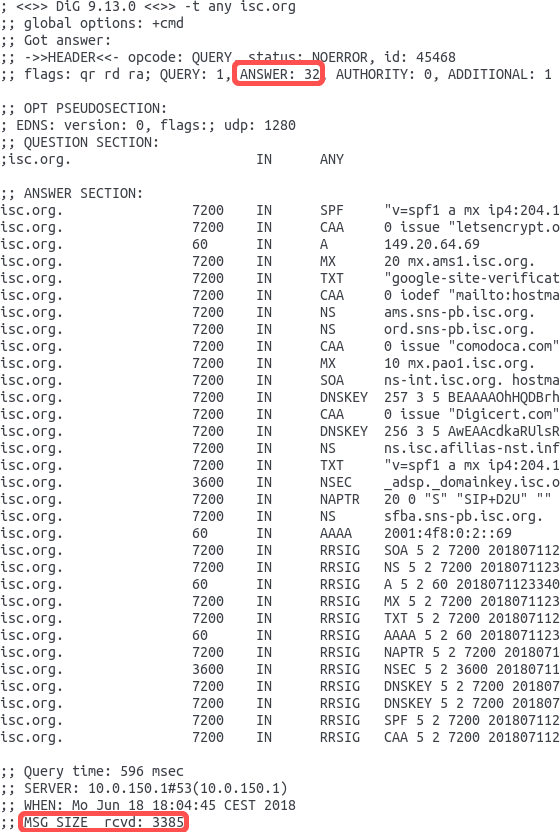
\includegraphics[width=10cm]{dig-dnsamplification}
    \caption{DNS Amplification am Beispiel von isc.org}
    \label{Analyse:DNS Amplification am Beispiel von isc.org}
  \end{figure}
  
\clearpage

Dies führt zu einem \ac{BAF} von ca. 56. Die folgende Grafik stellt einen Angriff mit diesem \ac{BAF} dar. Auf der X-Achse ist die Anzahl der gesendeten Pakete dargestellt, die Y-Achse zeigt die Last des Netzwerkes in Gigabit auf. Die Kurven beschreiben das Netz des Angreifers sowie des Opfers.

\begin{figure}[h]
    \centering
    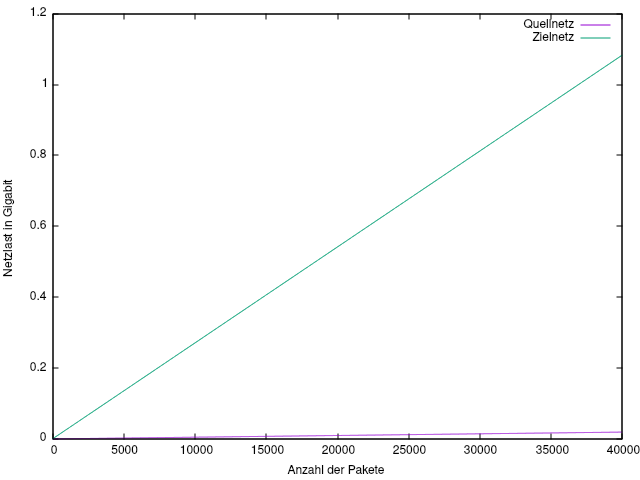
\includegraphics[width=15cm]{gnuplot-dnsamplification}
    \caption{Netzlast bei DNS Amplification}
    \label{Analyse:Netzlast bei DNS Amplification}
  \end{figure}
  
\clearpage

Auf der Darstellung ist zu erkennen, dass bei diesem Angriff eine lineare Steigerung der Netzlast in beiden Netzen vorliegt. Entscheidend ist jedoch der \ac{BAF}, welcher das Verhältnis zwischen der Lastzunahme im Angreifer- und Opfernetz beschreibt. Es ist zu erkennen, dass beim Versandt von 35000 Paketen im Quellnetzwerk nur ca. 0.016 Gigabit Daten transferiert werden müssen, dafür aber knapp 1 Gigabit an Daten in das Zielnetzwerk übertragen werden und dort für eine erhebliche Last sorgen.

Der \ac{DNS} bietet weitere Angriffsmöglichkeiten wie \ac{DNS} Fast Fluxing oder \ac{DNS} Information Leakage. Diese Angriffe dienen zum \textit{Phishing} von Daten oder der Spionage der Netzwerkstruktur. Sie nehmen initial keinen Einfluss auf den Netzwerkverkehr und dienen der Vorbereitung von Folgeangriffen und dem Sammeln von Informationen. Die Angriffsformen werden in \cite{Ledermueller2009} näher beschrieben. Die Analyse der Sicherheit der Netzwerkkommunikation beschränkt sich auf Angriffe, welche direkten Einfluss in die Kommunikation im Netzwerk haben. Weitere Formen der \ac{DoS}/\ac{DDoS} Angriffe finden auf Transportschicht \autoref{Analyse:Transportschicht} durch \textit{SYN-Flooding} oder auf Anwendungsschicht \autoref{Analyse:Anwendungsschicht} zur Negierung eines Speziellen Dienstes statt.

TODO - Schutzmaßnahmen sind DNSSEC und zufällige Informationen \label{Analyse:DNSSEC}
TODO - Die Auswirkungen eines solchen Angriffs ...
TODO - Sicherheitsmaßnahmen siehe \cite{Ledermueller2009}

\subsection{\ac{DHCP}}
\label{Analyse:DHCP}
\ac{DHCP} ist von der \ac{IETF} im \ac{RFC} 2131\footnote{Link - https://www.ietf.org/rfc/rfc2131.txt} definiert. Es stellt ein Framework zur Bereitstellung von \textit{Host} Konfigurationsparamertern in einem \ac{TCP}/\ac{IP} Netzwerk dar. Dazu gehören die \ac{IP} Adresse, Netzmaske, Gateway sowie zuständiger \ac{DNS} des Clients. Da ein neuer Client im Netzwerk keine Informationen über die vorhandenen Clients und dessen Topologie besitzt, muss er, um die Konfigurationsparameter für das Netzwerk zu erhalten (\ac{DHCP} Discover), über einen Broadcast im Netz nach Adress-Angeboten fragen. Dieser findet über das Transportprotokoll \ac{UDP} statt über die Ports 67 (Server) und 68 (Client) statt.

Der Mangel an Informationen bei der initialen Verbindung eines Clients im Netzwerk, kann von einem Angreifer genutzt werden, um die Netzwerkkonfiguration zu manipulieren. Da der Broadcast des Clients an das gesamte Netzwerk versandt wird, ist es dem Angreifer möglich selbst auf diese Anfrage zu antworten. Hierzu wird die Technik des Spoofing in Verbindung mit \ac{ARP} Poisoning oder einem zusätzlichen \ac{DHCP} Server (Rogue \ac{DHCP}), welcher vom Angreifer kontrolliert wird, im Netzwerk genutzt. In diesem Fall muss es dem Angreifer nur gelingen schneller auf den \ac{DHCP} Discover bzw. \ac{DHCP} Request des Clients zu antworten als der zuständige \ac{DHCP} Server. Somit ist es möglich die Netzwerkkonfiguration des Clients zu manipulieren.

In Kapitel \autoref{Impl:DHCP Spoofing} wird die Erweiterung des Testsystems (\cite{Weber2018}) um einen zusätzlichen \ac{DHCP} Server im Netzwerk durchgeführt, um mögliche Auswirkungen auf den Netzwerkverkehr an einem praktischen Beispiel darzustellen. Durch die Implementierung eines weiteren \ac{DHCP} Servers im Netzwerk wird ein Eingriff auf das Netzwerk in der Netzzugangsschicht und die gleichzeitige Manipulation des \ac{DHCP} der Anwendungsschicht des \ac{TCP}/\ac{IP} Referenzmodells beschrieben.

Ein Angriff auf das \ac{DHCP} in Netzwerken kann weitreichende folgen für die Netzwerksicherheit mit sich bringen. Durch die Änderung der Client-Adressen und Subnetze kann es zu \ac{IP} Adresskonflikten im Netzwerk kommen oder die Kommunikation beschränkt bzw. stillgelegt werden. Weitreichendere Auswirkungen auf die Netzwerksicherheit stellt das Umlenken des Datenverkehrs durch Manipulation der \ac{DNS}- bzw. Gateway-Parameter dar. Hierbei kann der gesamte Netzwerkverkehr eines Clients umgelenkt werden, um einen \ac{MitM} Angriff durchzuführen und den Netzwerkverkehr auszulesen.

Da das \ac{IP} Hilfsprotokoll \ac{DHCP} keine Sicherheitsmaßnahmen zur Verhinderung dieser Angriffe mit sich bringt, ist es notwendig sich vor diesen Bedrohungen schon auf den unteren Schichten des \ac{TCP}/\ac{IP} Referenzmodells zu schützen. Eine in der Industrie weit verbreitete Technik zum verhindern von Angriffen auf das \ac{DHCP} wird bereits in der Netzzugangsschicht umgesetzt. Netzwerkkomponenten wie Router und Swichtes werden mit Hilfe von \ac{DHCP} Snooping konfiguriert, welches es ermöglicht \ac{DHCP} Nachrichten zu überwachen und diese nur von vertrauenswürdigen Ports in das Netzwerk weiterzuleiten. Somit werden \ac{DHCP} Pakete, welche von einem im Netzwerk eingeschleusten Rogue-DHCP im Netzwerk verteilt werden sollen direkt verworfen und nehmen keinen Einfluss auf das bestehende Netzwerk.

\subsection{\ac{OPC UA}}
\label{Analyse:OPCUA}
Die Kommunikation zwischen \ac{OPC UA} Komponenten findet auf der Anwendungsschicht des \ac{TCP}/\ac{IP} Referenzmodells statt. \ac{OPC UA} stellt eine vertikale Verbindung der Kommunikationspartner auf allen Ebenen der Automatisierungspyramide her. Aufgrund der Öffnung von Unternehmen nach außen, den immer höheren Informationsbedarf und die direkte Kommunikation mit Händler und Kunden ist \ac{OPC UA} ein attraktives Ziel für Industriespionage und Sabotage des Netzwerks (\cite{opcpt2}). 

\ac{OPC UA} wurde als Client-Server Architektur entwickelt. Um \ac{OPC UA} auch in Systemen der unteren Ebenen der Automatisierungspyramide, wie Kleinsteuerungen, Sensoren und Low-End-Embedded-Systeme, einsetzen zu können, werden meist geringe Latenzen in den Netzwerken und ein geringer Overhead aufgrund von Ressourcenmangel sowie die Kommunikation mit mehreren Partnern benötigt. Diese Anforderungen werden von dem im Jahr 2018 veröffentlichten 14 Teil der \ac{OPC UA} Spezifikation \textit{Publish Subscribe} adressiert. Das \textit{Publish Subscribe} Modell wird mit Hilfe des Transportprotokolls \ac{UDP} umgesetzt und ermöglicht den Multi- und Broadcast sowie die Möglichekit der häufigen Übertragung von kleinen Datenmengen um \textit{Logging} oder \textit{Monitoring} durchzuführen, ohne das Netzwerk durch einen 3-Wege-Handshake bei jedem Verbindungsaufbau zusätzlich zu belasten (\cite{opcpt1}).

Aus zeitlichen Gründen wird sich im weiteren Verlauf der Thesis auf die Sicherheit der Netzwerkkommunikation im etablierten \ac{OPC UA} \textit{Client Server} Modell beschränkt.

Die \ac{OPC UA} beschreibt ein mehrschichtiges Sicherheitskonzept, welches \textit{Transport Layer-} und \textit{Application Layer Security} umfasst. Die \textit{Transport Layer Security} stellt die Sicherheit auf Nachritenebene her und beinhaltet \textit{Application Authentication}, \textit{Integrity} und \textit{Confidentiality}. Um dies zu ermöglichen, werden verschiedene Transport- sowie Anwendungsprotokolle im Verbund genutzt. Die Sicherheit auf Anwendungsebene stellt weitere Sicherheitsmechanismen zur \textit{Availability}, \textit{Auditing}, \textit{User Authorization} und \textit{User Authentication} bereit.

\subsubsection{Transport Layer Security}
Die \ac{OPC UA} beschreibt mit dem \ac{UACP} ein abstraktes Protokoll zur Herstellung einer Vollduplexverbindung in einer Client-Server Architektur. Implementierungen dieses Protokolls können über jede Middleware, welche den Austausch von Nachrichten im Vollduplexverfahren über \ac{TCP}/\ac{IP} und \textit{Websockets} unterstützt, durchgeführt werden. Somit ist das von \ac{OPC UA} spezifizierte Protokoll für die Zukunft flexibel. Die Spezifikation des abstrakten Protokolls \ac{UACP} wird im 5. Teil der \ac{OPC UA} Spezifikation\footnote{OPC Unified Architecture Specification Part 6: Mappings (\cite{opcpt5})} beschrieben und beinhaltet die Form der Nachricht, den Verbindungsaufbau, die Kommunikation und die Fehlerbehandlung.

In \autoref{Kap2:OPC UA Kommunikationswege} ist dargestellt, dass \ac{OPC UA} verschiedene Protokollestacks für unterschiedliche Anforderungen zur Kommunikation zwischen den Komponenten bereitstellt. Diese bestehen aus einer Verbindung von \ac{TCP} auf Transportebene und dem \ac{UA} Binary Protokoll zur Kodierung der Nachrichten, einem Webservice über \ac{HTTP}/\ac{HTTPS} und \ac{SOAP} mit \ac{XML} Encoding oder einer hybriden Form aus beiden. Alle Kommunikationsformen beinhalten ein Sicherheitsmodell auf Transport- oder Nachrichtebene.

\begin{figure}[h]
  \centering
  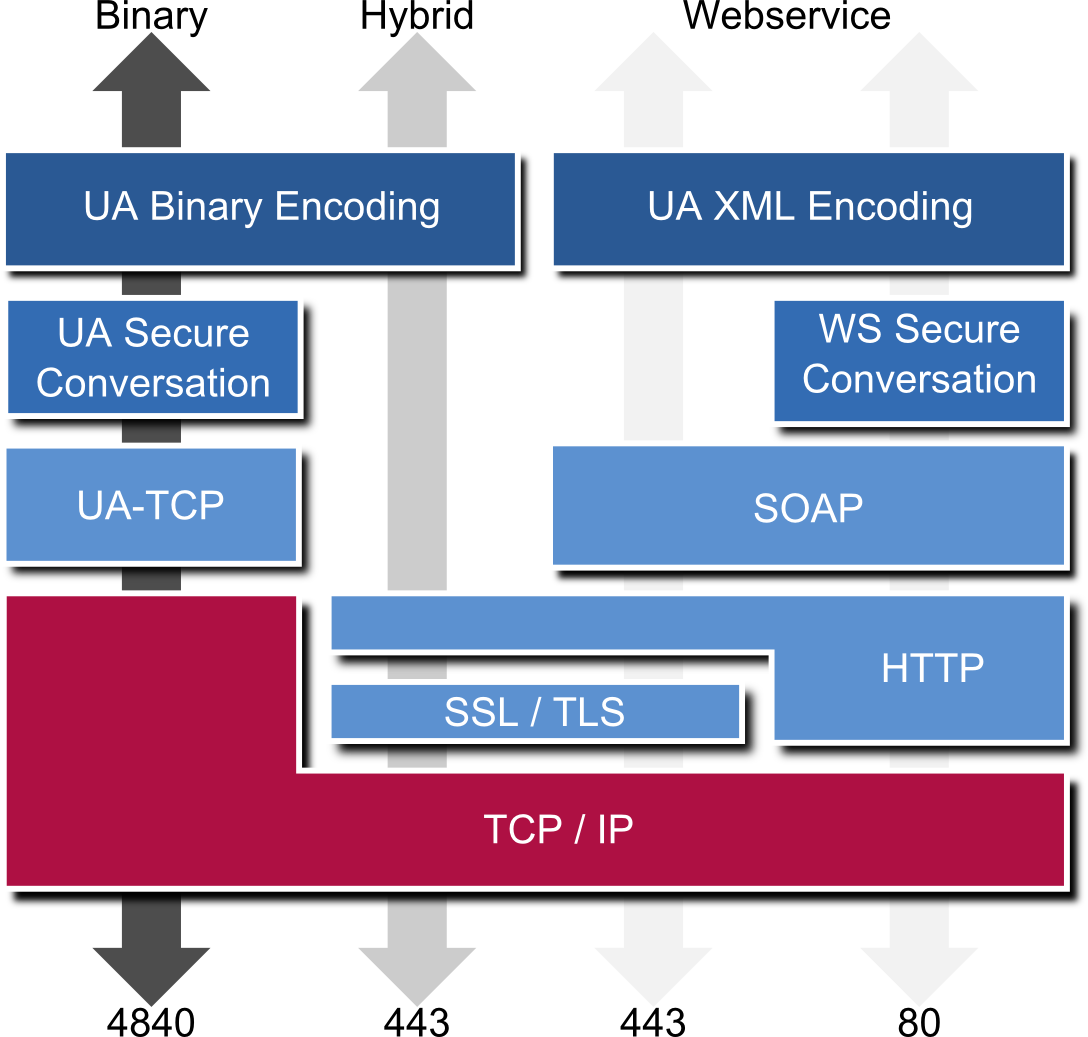
\includegraphics[width=10cm]{opcuaprotocol}
  \caption{OPC UA Kommunikationswege} 
  \label{Kap2:OPC UA Kommunikationswege}
\end{figure}

\clearpage

Die beschriebenen Protokollstacks bilden mit ihren Sicherheitsmechanismen die Grundlage für eine sichere Datenübertragung. Die Form der Datenübertragung über \ac{SOAP}/\ac{HTTP} wurde ab Version 1.03 der Spezifikation als veraltet angesehen, da es in der Industrie nicht umgesetzt wurde (\cite{opcpt5}). Die Protokolle \ac{UA} Binary über \ac{TCP} und die Hybridform aus den Protokollen \ac{UA} Binary und \ac{HTTPS} Webservice werden im folgenden auf ihre Standhaftigkeit bzgl. der Sicherheitsanforderungen in Industrie 4.0 Umgebungen analysiert.

\subsubsection{\ac{UA} Binary über \ac{TCP}}
Das \ac{UA} Binary Protokoll über \ac{TCP} wird für Kommunikation mit optimierter Geschwindigkeit und Durchsatz genutzt. Es besitzt den geringsten Overhead sowie Ressourcenverbrauch, da kein zusätzlicher Parser für \ac{HTTP} oder \ac{XML} genutzt werden muss und somit die Systemlast gering gehalten werden kann. Zur Kommunikation wird standardmäßig der Port 4840 genutzt. Die sichere Kommunikation wird erst auf Nachrichtenebene durch die \ac{UA} Secure Conversation hergestellt (siehe \autoref{Analyse:Application Layer Security}). Für die Transportebene gelten durch das genutzte Protkoll \ac{TCP} weiterhin die Bedrohungen von \autoref{Analyse:TCP}.

\subsubsection{\ac{UA} Binary über \ac{HTTPS}}
Die Hybridform der Kommunikation über einen \ac{HTTPS} Webservice mit Hilfe der \ac{UA} Binary Protokolls vereint die Vorteile des Ressourcenschonenden \ac{UA} Binary Protokolls über \ac{TCP} und die weitreichende Kompatibilität eines Webservice. Die Sicherheit der Netzwerkkommunikation wird bereits auf der Transportebene mit Hilfe von \ac{TLS} hergestellt.

Die Transportsicherheit wird mit \ac{TLS} 1.2 und der Cipher Suite \textit{TLS RSA WITH AES 256 CBC SHA256} bereitgestellt (\cite{opcpt7}). Hierbei ist zu beachten, dass die Rechenleistung der Systeme wächst und somit Verschlüsselungsalgorithmen mit der Zeit unsicher werden. Eine \ac{TLS} Verbindung mit schwacher Cipher Suite stellt keine sichere Verbindung bereit. Des Weiteren wurden in den Implementierungen von \ac{TLS} Fehler verursacht, welche die Transportsicherheit wie z. B. im Falle von \textit{Heartbleed}\footnote{Link zu Heartbleed} verhinderten.

Eine weitere Bedrohung stellt das genrelle Verfahren der Ausstellung von Zertifikaten bereit. Diese Zertifikate werden von Dienstleistern ausgestellt, welche als vertrauenswürdig eingestuft und als Root-\ac{CA} bezeichnet werden. Die Herstellung der Vertrauenswürdigkeit eines Ausstellers liegt im Ermessen des Softwareherstellers und dessen Aufnahme in die Liste vertrauenswürdiger \ac{CA}.

TODO - zu dünn

Die Kommunikation des Protokolls \ac{OPC UA} über Webservices und \ac{HTTP} bzw. \ac{HTTPS} wird im Rahmen dieser Thesis nicht weiter bearbeitet, da die Implementierung des im Testsystem genutzten NodeJS Moduls node-opcua unvollständig ist.

\subsubsection{Application Layer Security}
\label{Analyse:Application Layer Security}
\ac{OPC UA} stellt aufgrund der verschiedenen Anforderungen der Industrie an ihre Systeme mehrere Sicherheitskonfigurationen zur Informationsübertragung zur Verfügung. Dies ist notwendig, da die Verwendung von Verschlüsselungsalgorithmen und Kodierungsverfahren Ressourcen benötigt und Latenzen verursacht, welche unter Umständen nicht vorhanden sind oder nicht geleistet werden können. Eine Fehlkonfiguration des Protokolls kann jedoch auch Auswirkungen auf den Betrieb des Netzwerks und der Komponenten haben sowie die Integrität der Daten gefährden.

\ac{OPC UA} verifiziert vor dem Austausch von Nachrichten zwischen zwei Komponenten, ob ein SecureChannel vorhanden ist, über welchen die Daten übertragen werden. Dieser wird vom bestehenden Netzwerkstack und den genutzten niedrigeren Protokollen bereitgestellt (\cite{opcpt1}). Die \ac{UA} Secure Conversation besteht aus dem \textit{Secure Channel} und der Session und desssen gesetzten \textit{SecurityMode} (\cite{opcpt2}). Die Form der Nachrichten im \textit{Secure Channel} wird durch den in der gewählen \textit{Security Mode} bestimmt. Bei der Verwendung der \textit{Security Policy} None wird ein \textit{Secure Channel} hergestellt, welcher jedoch keine Sicherheitsprofile bereitstellt (\cite{opcpt7}). Dies wird in \autoref{Analyse:OPC UA Secure Channel} dargestellt.

\begin{figure}[h]
  \centering
  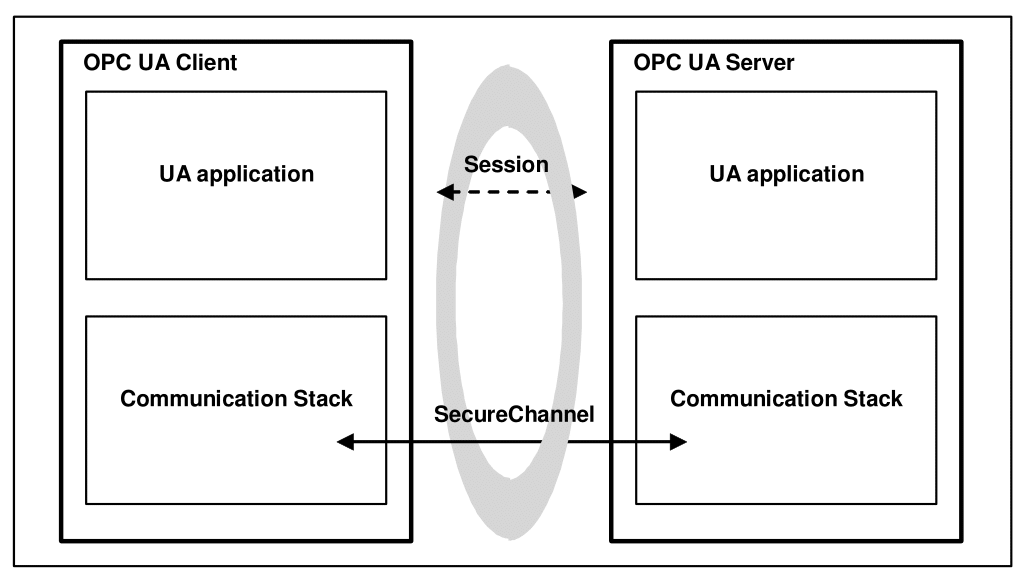
\includegraphics[width=10cm]{opcua-securechannel}
  \caption{OPC UA Secure Channel} 
  \label{Analyse:OPC UA Secure Channel}
\end{figure}

\clearpage

Mit Hilfe des vorhandenen Testsystems (\cite{Weber2018}) kann dieses Verhalten nachgewiesen werden. Hierfür wurde das Netzwerkanalysetool Wireshark\footnote{TODO - WIRESHARK} genutzt, um an der Netzwerkbrücke der Docker Container den Netzwerkverkehr zwischen den Komponenten abzuhören. In Verbindung mit dem \ac{OPC UA} \textit{Secure Channel} wurde das System erweitert, um verschiedene Sicherheitsprofile für die Kommunikation bereitzustellen. Die Erweiterung des Systems wird in \autoref{Impl:Analyse:OPC UA Secure Channel} beschrieben.

Die folgenden Abbildungen zeigen die Ergebnisse der Paketanalyse mit der vorhandenen \text{Security Policies} "none". Der \ac{OPC UA} Client des Control Containers, welcher die Liste der im Netzwerk vorhandenen \ac{OPC UA} Server abfrägt besitzt die \ac{IP}-Adresse 172.18.0.6, der Container des Discoveryservers die \ac{IP}-Adresse 172.18.0.2. In \autoref{Analyse:opcua-secure-none-req} ist der Request des Control Containers zum Aufbau eines \textit{Secure Channel} dargestellt. Die verwendete \textit{Security Policy} ist im Bereich SecurityPolicyUri des \ac{OPC UA} Protokolls beschrieben. In \autoref{Analyse:opcua-secure-none-res} ist die Antwort des \ac{OPC UA} Discoveryservers im \textit{Secure Channel} dargestellt. 

\begin{figure}[h]
  \centering
  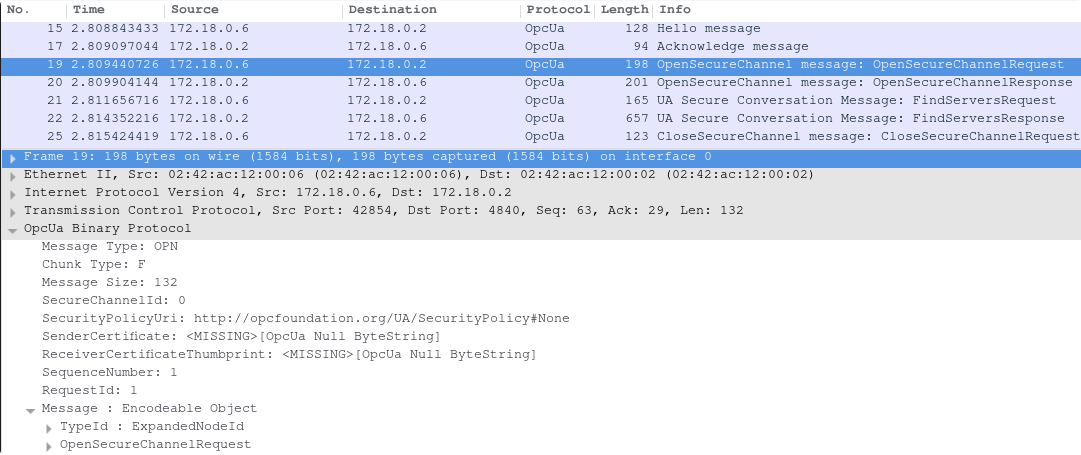
\includegraphics[width=15cm]{opcua-secure-none-req}
  \caption{Paketanalyse OPC UA - Client Request bei Sicherheitsprofil "none"} 
  \label{Analyse:opcua-secure-none-req}
\end{figure}

\begin{figure}[h]
  \centering
  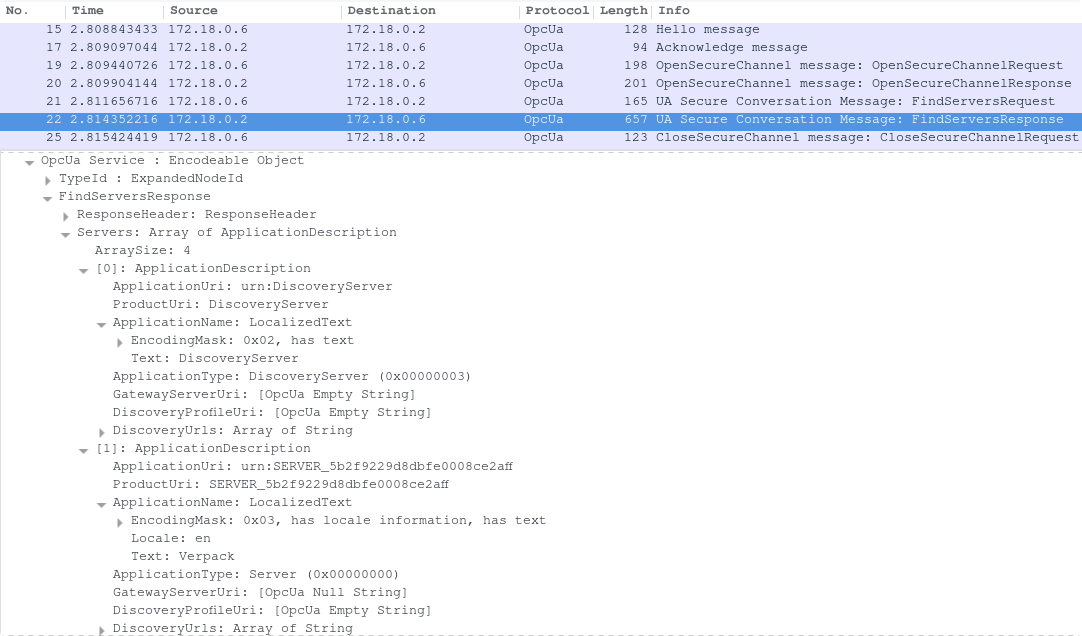
\includegraphics[width=15cm]{opcua-secure-none-res}
  \caption{Paketanalyse OPC UA - Server Response bei Sicherheitsprofil "none"} 
  \label{Analyse:opcua-secure-none-res}
\end{figure}

\clearpage

Es ist zu erkennen, dass die Kommunikation, obwohl der \textit{Secure Channel} genutzt wird, nicht verschlüsselt ist. Die Endpunkte sowie deren Adressen und bereitgestellte Methoden können aus den Paketen ausgelesen werden.

Im Folgenden wird erneut das Abfragen des Control Containers aller im Netzwerk vorhandenen Endpunkte beim Discoveryserver beschrieben, jedoch wird das Sicherheitsprofil "Basic256Sha256" mit dem \textit{MessageSecurityMode} "SIGNANDENCRYPT" genutzt. Der \ac{OPC UA} Client besitzt die \ac{IP}-Adresse 172.18.0.7. Der Discoveryserver weiterhin die Adresse 172.18.0.2. \autoref{Analyse:opcua-secure-sha-req} zeigt den Request, \autoref{Analyse:opcua-secure-sha-res} die verschlüsselte Response im \textit{Secure Channel}.

\begin{figure}[h]
  \centering
  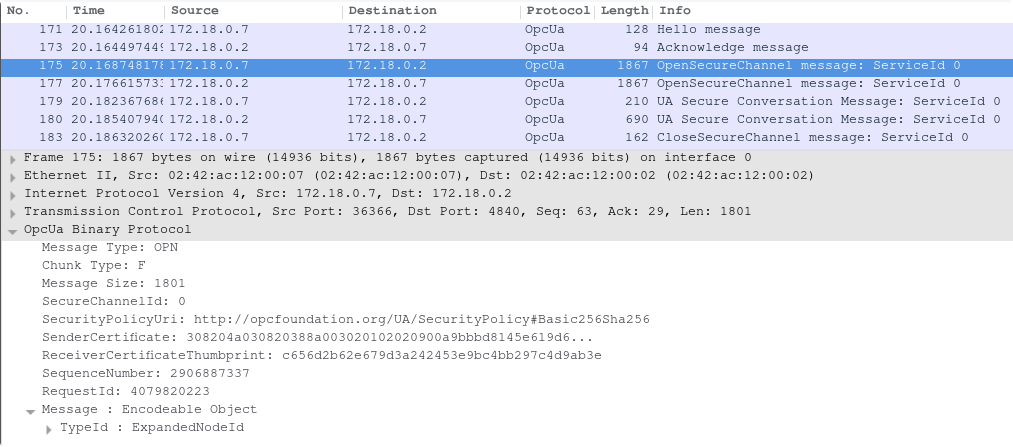
\includegraphics[width=15cm]{opcua-secure-sha-req}
  \caption{Paketanalyse OPC UA - Client Request bei Sicherheitsprofil "Basic256Sha256" und MessageSecurityMode "SIGNANDENCRYPT"} 
  \label{Analyse:opcua-secure-sha-req}
\end{figure}

\begin{figure}[h]
  \centering
  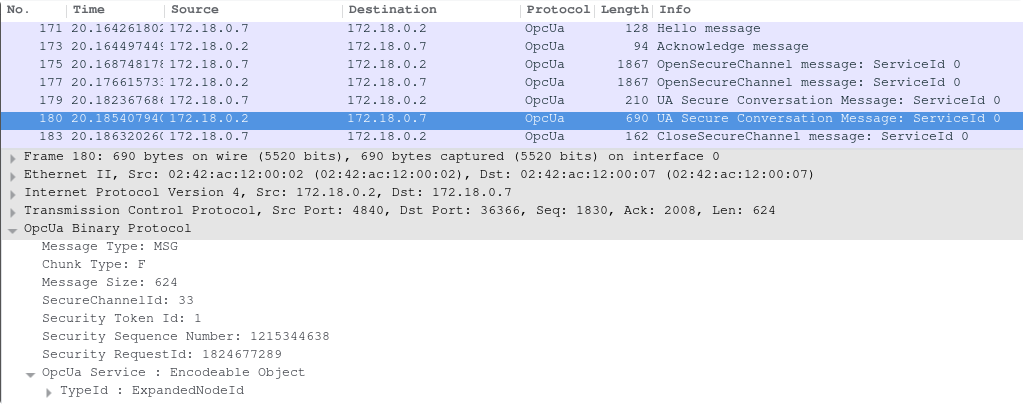
\includegraphics[width=15cm]{opcua-secure-sha-res}
  \caption{Paketanalyse OPCUA - Server Response bei Sicherheitsprofil "Basic256Sha256" und MessageSecurityMode "SIGNANDENCRYPT"} 
  \label{Analyse:opcua-secure-sha-res}
\end{figure}

\clearpage

Es ist zu erkennen, dass der gesamte Netzwerkverkehr im \textit{Secure Channel} durch ein Zertifikat signiert sowie durch den Algorithmus SHA256 verschlüsselt wurde. Die Integrität und Vertraulichkeit während der Kommunikation im Netzwerk ist gewährleistet.

Es ist zu Beachten, dass - TODO Rechenleistung erhöht sich -> Verschlüsselungsalgorithmen werden unsicher -> OPC ist flexibel für zukunft und anforderungen

\subsubsection{weitere Sicherheitsbestandteile}
TODO - PKI 
TODO - Zertifikatsmanagement 
TODO - Zeitsynchronisation
TODO - Kerberos OAuth2
TODO - siehe BSI UPC UA Analyse

\subsection{\ac{MQTT}/\ac{CoAP}}
TODO - Ansatz: Wireshark an Bridge der Testumgebung im Sternnetzwerk und Druckerkomponente oder andere manipulieren; andere Protokolle von Feldebene an Switch auslesen; vielleicht hier nur beschreiben und in den höheren Schichten durchführen mit CoAP oder MQTT -> OPC UA Komponenten sind Gateway

\section{Schutzmaßnahmen}
TODO - Applikationssicherheit != Netzwerksicherheit != Betriebssystemsicherheit

\subsection{allgemeine Schutzmaßnahmen}
TODO - Schutz auf allen Ebenen -> z.B. OPC UA basiert auf IP-Netz -> Angriffsvektoren von IP und genutzten Diensten immer noch zutreffend

\subsection{TODO}
\subsection{TODO}

\subsection{Defense in Depth}
Auf der Netzzugangsschicht fallen, wie auf allen anderen Schichten, Betriebsdaten an, welche genutzt werden können, um Angriffe oder unregelmäßige Aktivitäten im Netzwerk zu erkennen. Es kann protokolliert werden, wann ein Gerät mit den Netzwerk verbunden war und welche Pakete andere Netzwerkteilnehmer von diesem Gerät erhalten haben (\cite{sichKom2017}). Die Norm IEC 62443\footnote{ref. IEC 62443} definiert die Defense in Depth Strategie. Sie stellt ein Konzept bereit, um die IT-Sicherheit der Anlagen, die Netzwerksicherheit und Systemintegrität nach dem Stand der Technik zu schützen. Sie gliedert eine Unternehmensinfrastruktur in multiple und redundante Sicherheitsschichten (Zonen), um ein höchstmögliches Sicherheitsniveau zu erreichen. Die unabhängigen Verteidigungslinien sollen Angriffe verzögern, um Zeit für Gegenmaßnahmen zu gewinnen. Die Kommunikation erfolgt in separierten Netzsegmenten, welche zusätzlich mit \ac{IDS} nutzen, um Angriffe schnell zu erfassen und Gegenmaßnahmen einleiten zu können. Somit wird der Aufwand, um die unteren Netzwerkebenen zu kompromittieren durch den Einsatz von \ac{DMZ}, \ac{IDS}, Paketfilter und Time Access Control wesentlich erhöht. Zusätzlich ist das "`Zone and Conduit"' Modell eines der zentralen Elemente der Defense in Depth Strategie. Die verschiedenen Zonen können nur mittels spezieller Leitungen (Conduits) miteinander kommunizieren.  

\begin{figure}[h]
    \centering
    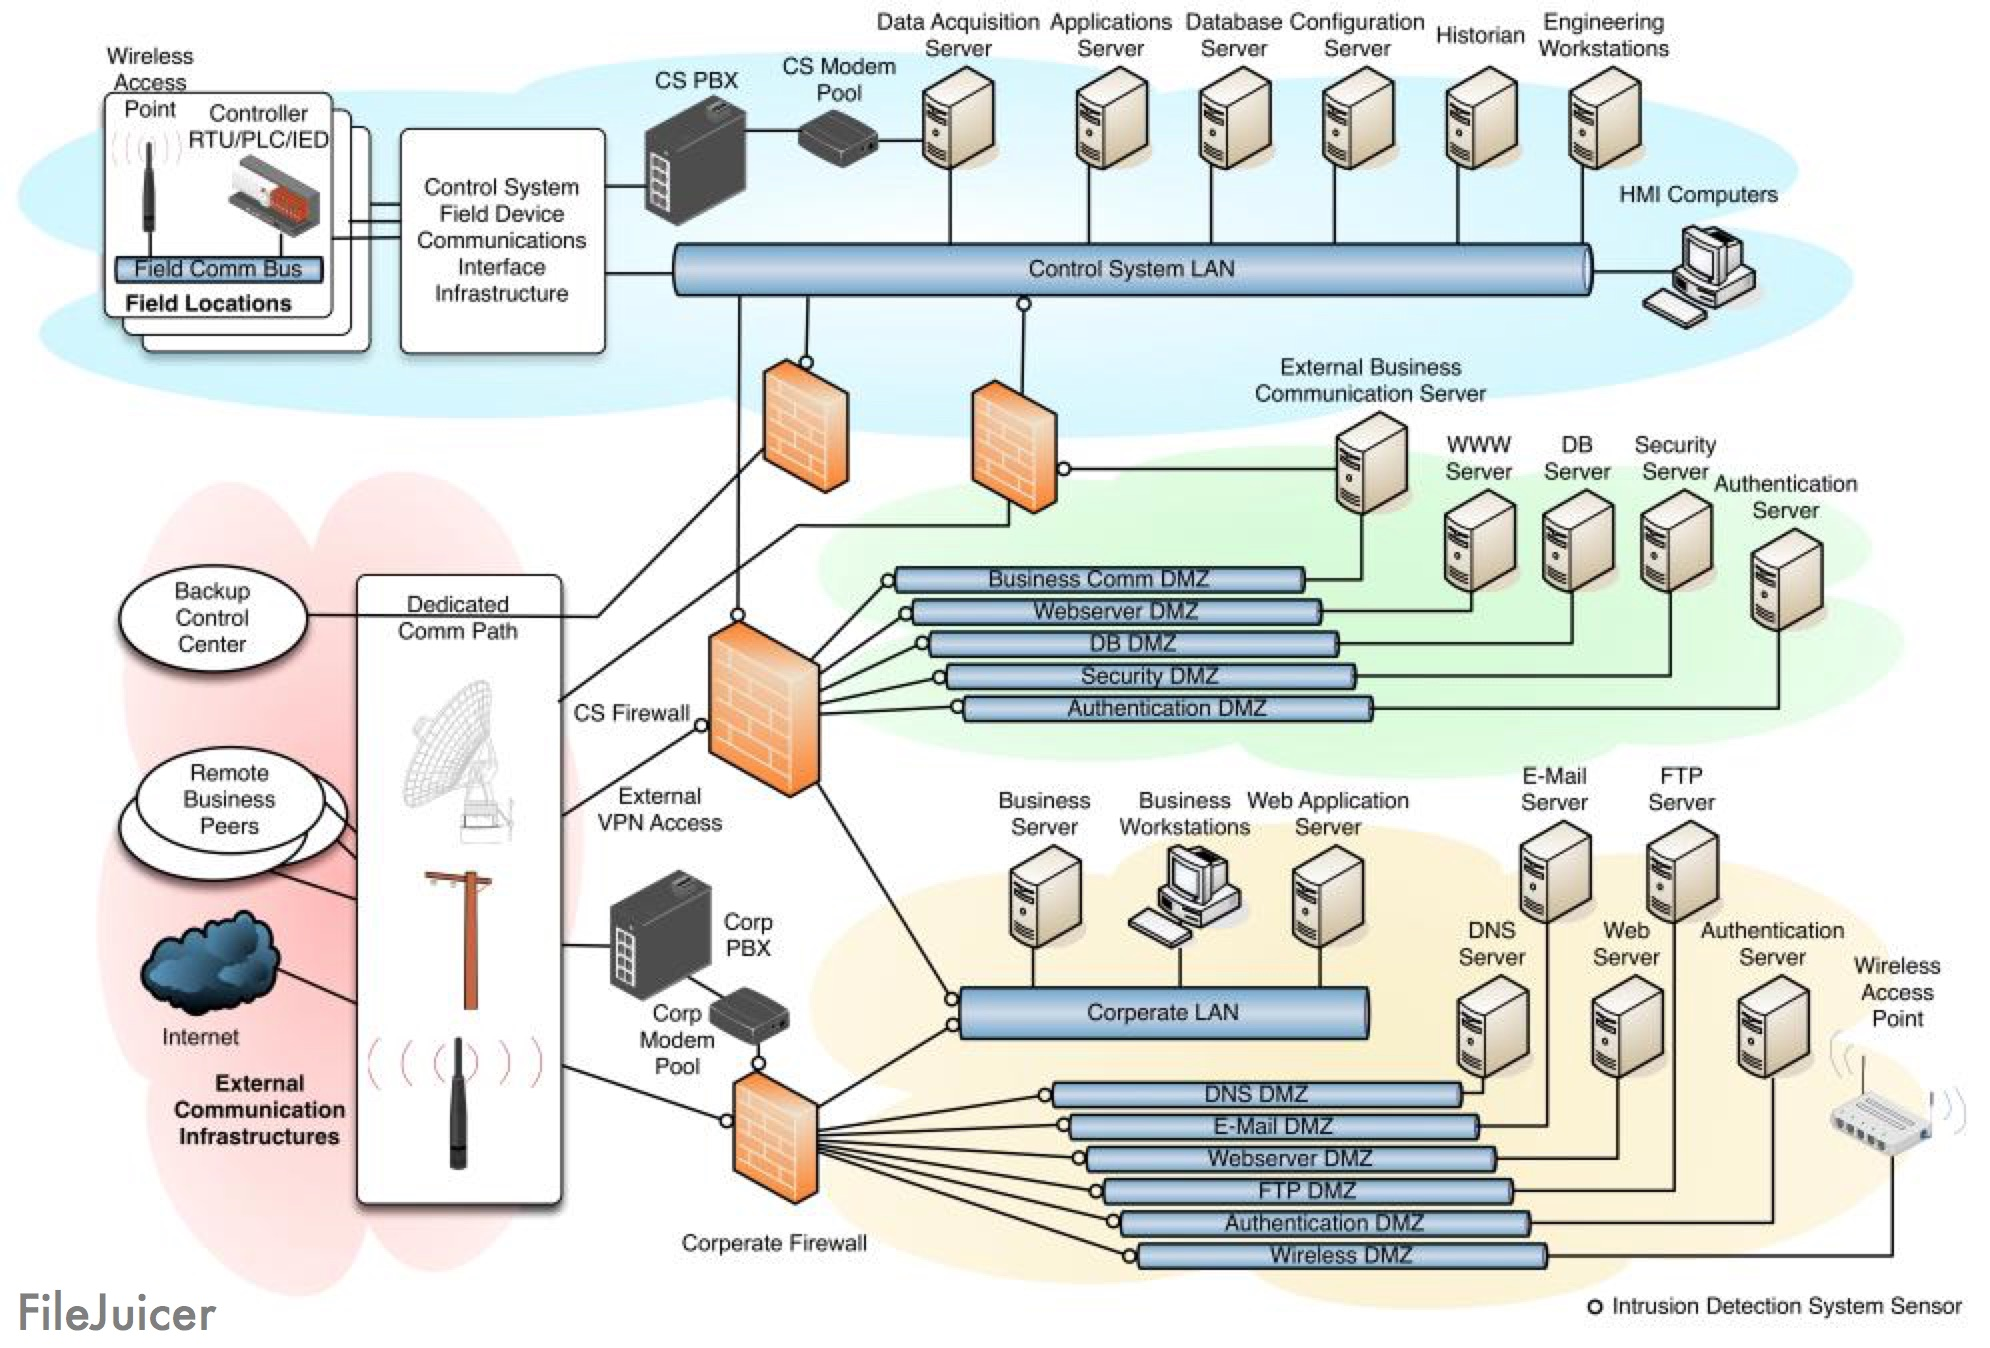
\includegraphics[width=15cm]{defense-in-depth-strategie}
    \caption{Defense in Depth Strategie - \cite{kuipers2006}}
    \label{Kap3:Defense-in-Depth}
\end{figure}

\clearpage

Das Defense in Depth Konzept stellt ein Konzept dar, um Industrieanlagen und Unternehmensnetzwerke vor Angriffen zu schützen. Bei der sich ständig ändernden Bedrohungslage in den komplexen Netzen wird bei dieser Strategie jedoch weniger ein vollständiger Schutz bereitgestellt, als eine Strategie zur Schadensbegrenzung im Falle eines Angriffs.